 \section{Closure ODP}\begin{description}
\item [CLASSIFICATION:] Good Practice.

\item [MOTIVATION:] OWL sometimes is anti-intuitive due to the Open World Assumption. One of the examples of such problem is the fact that plenty of users think that asserting an existential restriction is enough to close a relationship, when in fact a universal restriction is also needed: it is not enough to say that carnivore eats some meat, as that is equivalent to saying that it can eat another things apart of meat.

\item [AIM:] Simulate the closed world assumption in a concrete class.

\item [STRUCTURE:] See Figure \ref{odp:Closure_abstract}.
\begin{figure}[]\centering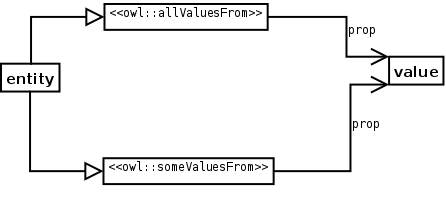
\includegraphics[width=\textwidth]{Catalogue/Closure_abstract}\caption{\label{odp:Closure_abstract} Abstract structure of the Closure ODP.}\end{figure}

\item [SAMPLE:] See Figure \ref{odp:Closure_instance}.
\begin{figure}[]\centering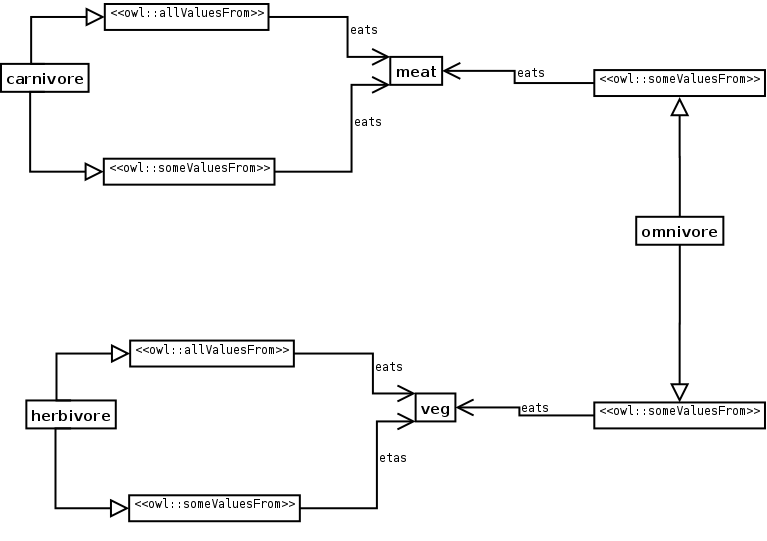
\includegraphics[width=\textwidth]{Catalogue/Closure_instance}\caption{\label{odp:Closure_instance} Sample structure of the Closure ODP.}\end{figure}

\item [ELEMENTS:] The only element to take into account is the object property that will be used to produce the closure.

\item [IMPLEMENTATION:] The only necessary step is to add an existential restriction and an universal restriction with the same filler.

\item [RESULT:] The closure axiom allows to close the world and express that something has got a property and only that property. For example, following the example, without the closure (without the universal restriction) carnivore and herbivore would appear as subclasses of omnivore. However, with the closure axiom, they do not.

\item [REFERENCES: ] ~\begin{itemize}
\item Explicit Knowledge Engineering Patterns with Macros. Denny Vrandecic.
In Proceedings of the Ontology Patterns for the Semantic Web Workshop (ISWC 2005).
\item Alan Rector, Nick Drummond, Matthew Horridge, Jeremy Rogers, Holger Knublauch,  Robert Stevens, Hai Wang, Chris Wroe. OWL Pizzas: Practical Experience of Teaching OWL-DL: Common Errors and Common Patterns. In Proceedings of  the European Conference on Knowledge Acquistion, 2004. LNCS- LNAI 3257, Springer-Verlag.pp 63-81.\end{itemize}
\item [URL: ] \url{http://www.gong.manchester.ac.uk/odp/owl/Good_Practice_ODP/Closure.owl} \end{description}